The research by \citep{RuizGarciaMiranda2007} provides a simple relationship for SDoF systems between inelastic displacement  and the corresponding median elastic spectral displacement value. The procedure presented herein is applicable to bilinear elasto-plastic capacity curve only and it can be used to estimate single building fragility curve. Moreover the fragility curves derived for single buildings can be combined in a unique fragility curve, which considers also the inter-building uncertainty.

The relationship provided by \citep{RuizGarciaMiranda2007} has been adapted for MDoF systems (\citep{Vamvatsikos2014}), relating the inelastic top displacement of a structure $\hat{d}_{roof}$ to the median elastic spectral displacement value at its fundamental period of vibration $\hat{S}_{d}(T)$, as presented in the following equation:

\begin{equation}
\hat{S}_d(T_1) = \frac{\hat{d}_{roof}}{\hat{C}_R \Gamma_1 \Phi_1} 
\label{eq:basic_DF}
\end{equation}

where $\Gamma_1 \Phi_1$ is the first mode participation factor estimated for the first-mode shape normalised by the roof displacement, and C$_R$ is the inelastic displacement ratio (inelastic over elastic spectral displacement), computed by \citep{RuizGarciaMiranda2007} for nonlinear SDoF systems, which is a function of the first-mode period of vibration and the relative lateral strength of the system R. Therefore the median spectral acceleration at the fundamental period of vibration $\hat{S}_{a}(T)$ turns out to be expressed as a function of top displacement according to the following equation:

\begin{equation}
\hat{S}_{a}(T) = \frac{4 \pi^2}{\hat{C}_R T^2 \Gamma_1 \Phi_1} \hat{d_{roof}}
\label{eq:Sa_RGM}
\end{equation}

Estimates of $\hat{C}_R$ parameter are provided by \citep{RuizGarciaMiranda2007}, as result of nonlinear regression analysis of three different measures of central tendency computed from 240 ground motions:

\begin{equation}
\hat{C}_R = 1 + \frac{\hat{R} - 1}{79.12 T_1 ^{1.98}}
\label{eq:Cr_RGM}
\end{equation}

where $\hat{R}$ is given by the following equation:

\begin{equation}
\hat{R} = max(0.425(1 - c + \sqrt{c^2 + 2c(2 \hat{\mu} - 1) + 1}),1)
\label{eq:R_RGM}
\end{equation}

where c = 79.12 T$^{1.98}$, and $\hat{\mu}$ is the median ductility level of interest.

Moreover \citep{RuizGarciaMiranda2007} provide an estimate of the dispersion of C$_{R}$ parameter due to record-to-record variability with Equation \ref{eq:beta_eq_RGM}, that can be assumed equal to the dispersion of $d_{roof}$, since the two quantities are proportional.

\begin{equation}
\sigma_{\ln(C_R)} = \sigma_{\ln(d_{roof})} = \beta_{\theta d} = 1.975 [\frac{1}{5.876} + \frac{1}{11.749 (T + 0.1)}] [1- \exp(-0.739 (R - 1))]
\label{eq:beta_eq_RGM}
\end{equation}

The median value of $S_a$ corresponding to any level of ductility ($d_{roof}/d_y$) can be defined combining Equation from \ref{eq:Sa_RGM} to \ref{eq:R_RGM}. The relationship between the 16$^{th}$ and 84$^{th}$ fractiles of $\mu$ and R can be drawn instead, computing $\beta_{\theta d}$ for a discretised number of R with eq. \ref{eq:beta_eq_RGM}, and calculating the 16$^{th}$ and 84$^{th}$ fractiles of $\mu$ ($\mu_{16\%}$ and $\mu_{84\%}$), according to the Equations \ref{eq:mu16-beta} and \ref{eq:mu84-beta}. $\mu_{16\%}$-$R_{50\%}$, $\mu_{50\%}$-$R_{50\%}$ obtained in such way are shown in Figure \ref{fig:Rmu}.

\begin{figure}[!htbp]
\centering
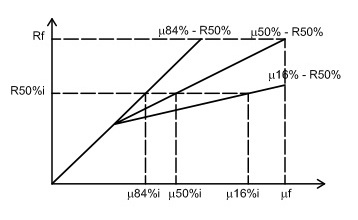
\includegraphics[width=8cm]{./figures/Rmu.jpg}
\caption{R-$\mu$ relationship.}
\label{fig:Rmu}
\end{figure}

For any inelastic displacement, and therefore any level of ductility $\mu$ the corresponding $R_{50\%}$, $R_{16\%}$, and $R_{84\%}$ values are found interpolating the aforementioned curves. Median R and its dispersion at ductility levels corresponding to the damage thresholds ds can thus be determined, and converted into median $S_{a, ds}$ and its dispersion due to record-to-record variability $\beta_{S_{a d}}$, according to equations \ref{eq:SaR} and \ref{eq:betaR}. 

If dispersion in the damage state threshold is different from zero, different values of ductility limit state are sampled from the lognormal distribution with median the median value of the ductility limit state, and dispersion the input $\beta_{\theta c}$. For each of these ductilities the corresponding $R_{50\%}$, $R_{16\%}$, and $R_{84\%}$ values are found interpolating the $\mu_{50\%}-R_{50\%}$, $\mu_{16\%}-R_50\%$ and $\mu_{84\%}-R_50\%$ curves, and converted into $\hat{S}_{a,ds}$ and $\beta_{S_{a d}}$ according to Equations \ref{eq:SaR} and \ref{eq:betaR}. MC random S$_a$ for each of the MC sampled ductility limit states are computed using $\hat{S}_{a,ds}$ and $\beta_{S_{a d}}$, and their median and dispersion are estimated. These parameters constitute the median $\hat{S}_{a,ds}$ and the total dispersion $\beta_{S_a}$ for the considered damage state. The procedure is repeated for each damage state.

If multiple buildings have been input to derive fragility function for a class of buildings all $\hat{S}_{a, blg}$ and $\beta_{S_a, blg}$ are combined in a single lognormal curve as described in section \ref{subsec:SPO2IDA}.\\

In order to use this methodology, it is necessary to load one or multiple capacity curves as described in Section \ref{subsec:cap_curves}. The pushover curve input type needs to be either Base Shear vs Roof Displacement (Section \ref{subsubsec:VB-Droof}), or Base Shear vs Floor Displacements (Section \ref{subsubsec:VB-Dfloor}). The capacity curves are then idealised with a bilinear elasto-plastic shape. If the user has already at disposal an idealised multilinear pushover curve for each building, the variable \verb=Idealised= in the csv input file should be set to \verb=TRUE=, and idealised curves should be provided according to what described in section \ref{subsec:cap_curves}. Then, it is necessary to specify a damage model using the parameter \verb=damage_model= (see Section \ref{subsec:dmg_model}).

If dispersion due to uncertainty in the limit state definition is different from zero a Monte Carlo sampling needs to be performed to combine it with the record-to-record dispersion. The number of Monte Carlo samples should be defined in the variable \verb=montecarlo_samples=.
After importing the module RGM2007, it is possible to calculate the parameter of the fragility model, median and dispersion, using the following command:

\begin{Verbatim}[frame=single, commandchars=\\\{\}, samepage=true]
fragility_model = RGM2007.calculate_fragility(capacity_curves, ...
idealised_capacity, damage_model, montecarlo_samples, Sa_ratios)
\end{Verbatim}

where \verb=Sa_ratios= is the spectral ratio variable, needed to combine together fragility curves for many buildings, as described in Section \ref{subsec:SPO2IDA}.